\documentclass[11pt,a4paper]{article}

\usepackage[margin=20mm,headheight=16mm,includeheadfoot]{geometry}
\usepackage{fontspec}
\setmainfont{Calibri}[
  Path = {/Applications/Microsoft Word.app/Contents/Resources/DFonts/},
  Extension = .ttf,
  UprightFont = Calibri,
  BoldFont = Calibrib,
  ItalicFont = Calibrii,
  BoldItalicFont = Calibriz
]
\setsansfont{Calibri}[
  Path = {/Applications/Microsoft Word.app/Contents/Resources/DFonts/},
  Extension = .ttf,
  UprightFont = Calibri,
  BoldFont = Calibrib,
  ItalicFont = Calibrii,
  BoldItalicFont = Calibriz
]
\usepackage{graphicx}
\usepackage{xcolor}
\usepackage{booktabs}
\usepackage{tabularx}
\usepackage{longtable}
\usepackage{array}
\usepackage{enumitem}
\usepackage{tikz}
\usetikzlibrary{arrows.meta,positioning,fit,backgrounds}
\usepackage{fancyhdr}
\usepackage{hyperref}
\usepackage{microtype}
\setlength{\emergencystretch}{2em}

\makeatletter
\renewcommand\section{%
  \@startsection{section}{1}{\z@}%
    {-2.4ex \@plus -1ex \@minus -.2ex}%
    {1.3ex \@plus .2ex}%
    {\Large\sffamily\bfseries\color{hcNavy}}%
}
\renewcommand\subsection{%
  \@startsection{subsection}{2}{\z@}%
    {-2.0ex \@plus -1ex \@minus -.2ex}%
    {0.7ex \@plus .2ex}%
    {\large\sffamily\bfseries\color{hcInk}}%
}
\renewcommand\subsubsection{%
  \@startsection{subsubsection}{3}{\z@}%
    {-1.6ex \@plus -1ex \@minus -.2ex}%
    {0.4ex \@plus .2ex}%
    {\normalsize\sffamily\bfseries\color{hcInk}}%
}
\makeatother

\definecolor{hcOrange}{HTML}{F15A24}
\definecolor{hcNavy}{HTML}{1B2430}
\definecolor{hcInk}{HTML}{243040}
\definecolor{hcMute}{HTML}{5C6770}
\definecolor{hcLine}{HTML}{E4E0DA}
\definecolor{hcWash}{HTML}{FFF6F1}

\hypersetup{
  pdftitle={Hutch Clarity MCP Interface Specification},
  pdfauthor={Hutch Clarity},
  pdfsubject={Model Context Protocol interface provided by Hutch Clarity},
  colorlinks=true,
  linkcolor=hcNavy,
  urlcolor=hcOrange,
  citecolor=hcNavy
}

\pagestyle{fancy}
\fancyhf{}
\fancyhead[L]{
\includegraphics[height=8mm]{assets/hutch-clarity-mark.png}\hspace{2mm}%
  {\sffamily\bfseries\color{hcNavy}Hutch Clarity}}
\fancyhead[R]{\sffamily\small\color{hcMute}HC-MCP-001}
\fancyfoot[L]{\sffamily\small\color{hcMute}MCP Interface Specification}
\fancyfoot[R]{\sffamily\small\color{hcMute}\thepage}
\renewcommand{\headrulewidth}{0.4pt}
\renewcommand{\headrule}{\hbox to\headwidth{\color{hcOrange}\leaders\hrule height \headrulewidth\hfill}}
\renewcommand{\footrulewidth}{0pt}

\setlist[itemize]{leftmargin=1.3em,itemsep=0.2em,topsep=0.3em}
\setlist[enumerate]{leftmargin=1.4em,itemsep=0.25em,topsep=0.3em}

\newcommand{\tool}[1]{\texttt{#1}}
\newcommand{\code}[1]{\texttt{#1}}

\begin{document}

\hypersetup{pageanchor=false}
\begin{titlepage}
\thispagestyle{empty}
\vspace*{6mm}

\includegraphics[width=92mm]{assets/hutch-clarity-logo.png}

\vspace{16mm}
{\sffamily\color{hcOrange}\bfseries\normalsize MODEL CONTEXT PROTOCOL}\\[3mm]
{\sffamily\color{hcNavy}\bfseries\fontsize{26}{30}\selectfont Interface Specification}\\[4mm]
{\color{hcOrange}\rule{42mm}{1.6pt}}\\[6mm]
{\sffamily\large\color{hcInk}Capabilities provided to a registered agent}

\vspace{12mm}
\begin{tabular}{@{}ll@{}}
\sffamily\color{hcMute}Document & \sffamily HC-MCP-001 \\[1.5mm]
\sffamily\color{hcMute}Version & \sffamily 1.0 \\[1.5mm]
\sffamily\color{hcMute}Status & \sffamily Issued \\[1.5mm]
\sffamily\color{hcMute}Date & \sffamily 5 October 2026 \\[1.5mm]
\sffamily\color{hcMute}Server & \sffamily \code{clarity} \\[1.5mm]
\sffamily\color{hcMute}Protocol & \sffamily MCP, 2026-07-28 \\
\end{tabular}

\vfill
{\sffamily\small\color{hcMute}
This document is the interface contract of \code{clarity-mcp}.\\
It states the tools, profiles, and controls the product provides.\\
A registered agent may read and propose. It may not execute.}
\vspace{8mm}
\end{titlepage}
\hypersetup{pageanchor=true}
\setcounter{page}{1}

\tableofcontents
\newpage

\section{Purpose}

Hutch Clarity explains a charge from system evidence, applies a remedy only when a versioned rule and the decision policy allow it, and issues a signed Trust Receipt for every executed plan.

\code{clarity-mcp} is the governed interface through which a registered agent uses those capabilities. The server name is \code{clarity}. The title presented to the client is Hutch Clarity. The server instruction is fixed:

\begin{quote}
\sffamily\color{hcInk}
Explain charges from evidence. Every answer must cite the case evidence or a rule. You cannot move money: the strongest action available is proposing a remedy the decision already allows, which a person or the customer then confirms.
\end{quote}

The agent receives tool contracts. It does not receive credentials, database access, or an execution path. Amounts, causes, and eligibility are produced by rule packs and the decision policy. The agent writes and reads language around those facts.

\section{What the product provides}

Through this interface a registered agent can:

\begin{itemize}
  \item read the evidence timeline of a case, including source completeness and the snapshot hash;
  \item read the cause assessment, the outcome, the ruled-out causes, and the actions the decision allows;
  \item read the plain description, legal basis, and required evidence of a published rule;
  \item read the public view of a Trust Receipt after one has been issued;
  \item read the safeguards recorded for the subscriber of a case;
  \item read the network status supplied for the subscriber of a case;
  \item search the published rule catalogue and receive cited passages;
  \item request a handoff to a person, with a reason code;
  \item propose one action the decision already allows, and receive a pending plan;
  \item on a staff session, read the desk queue ordered by money at stake.
\end{itemize}

Confirmation, approval, execution, receipt signing, bulk remedy, and policy publication are provided by other interfaces of the product. They are not tools on this server. Section~\ref{sec:outside} lists that boundary.

\section{Architecture}
\label{sec:architecture}

\code{clarity-mcp} is a separate deployable from the Clarity API. It speaks MCP over Streamable HTTP at \code{/mcp}. It holds no database. It is an OAuth~2.1 resource server only: it validates tokens and never issues them.

\begin{figure}[ht]
\centering
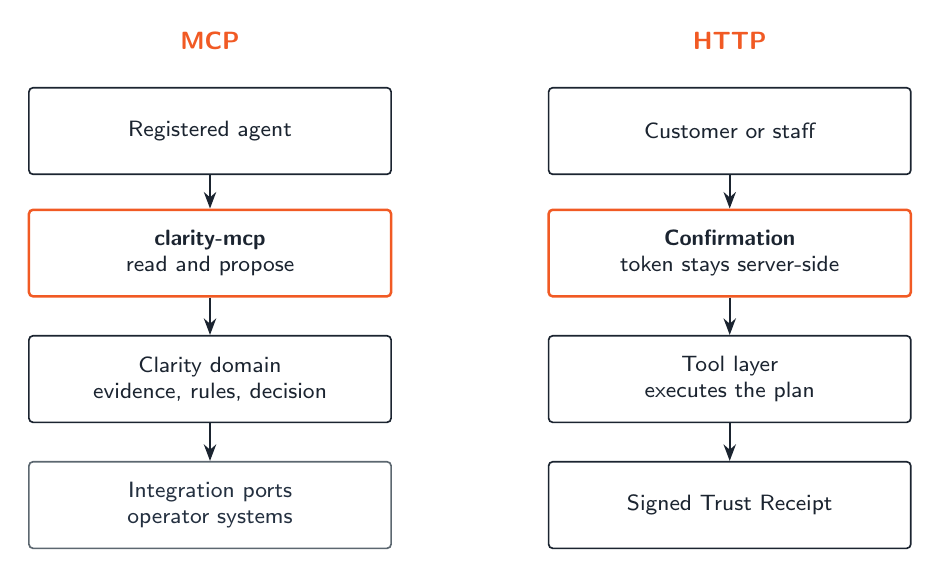
\begin{tikzpicture}[
  font=\sffamily\footnotesize,
  box/.style={draw=hcNavy, line width=0.6pt, rounded corners=1.5pt,
              align=center, inner sep=4pt, fill=white, text=hcNavy,
              minimum width=46mm, minimum height=11mm},
  accent/.style={box, draw=hcOrange, line width=0.9pt},
  quiet/.style={box, draw=hcMute, text=hcInk},
  arr/.style={-{Stealth[length=2.1mm]}, line width=0.7pt, hcNavy},
  lab/.style={font=\sffamily\small\bfseries\color{hcOrange}, fill=white, inner sep=1.5pt}
]
  \node[box] (agent) at (0,0) {Registered agent};
  \node[accent] (mcp) at (0,-1.55) {\textbf{clarity-mcp}\\read and propose};
  \node[box] (domain) at (0,-3.15) {Clarity domain\\evidence, rules, decision};
  \node[quiet] (ports) at (0,-4.75) {Integration ports\\operator systems};

  \node[box] (person) at (6.6,0) {Customer or staff};
  \node[accent] (confirm) at (6.6,-1.55) {\textbf{Confirmation}\\token stays server-side};
  \node[box] (tools) at (6.6,-3.15) {Tool layer\\executes the plan};
  \node[box] (receipt) at (6.6,-4.75) {Signed Trust Receipt};

  \draw[arr] (agent) -- (mcp);
  \draw[arr] (mcp) -- (domain);
  \draw[arr] (domain) -- (ports);
  \draw[arr] (person) -- (confirm);
  \draw[arr] (confirm) -- (tools);
  \draw[arr] (tools) -- (receipt);
  \node[lab] at (0,1.15) {MCP};
  \node[lab] at (6.6,1.15) {HTTP};
\end{tikzpicture}
\caption{Two doors. An agent reaches Clarity only through \code{clarity-mcp}. Execution is reached only after confirmation on the HTTP interface. The two paths do not join inside the agent.}
\label{fig:doors}
\end{figure}

A downstream call, where one is required, uses a new token obtained by RFC~8693 token exchange. The inbound client token is never forwarded. If token exchange is not configured, the downstream call is refused.

\section{Transport and protocol}

\begin{center}
\small
\begin{tabularx}{\textwidth}{@{}lX@{}}
\toprule
\textbf{Item} & \textbf{Provided value} \\
\midrule
Protocol & Model Context Protocol, revision 2026-07-28 \\
Transport & Streamable HTTP \\
Path & \code{/mcp} \\
Server name & \code{clarity} \\
Authentication & Bearer access token. A call with no token is refused (HTTP 401). \\
Resource indicator & RFC~8707. A token issued for another resource is refused. \\
Session state & Stateless. The server keeps no conversation memory. \\
\bottomrule
\end{tabularx}
\end{center}

Two MCP App resources are published for a host that can render them in a sandbox:

\begin{itemize}
  \item \code{ui://clarity/why-card}, the explanation card for a case;
  \item \code{ui://clarity/receipt}, the receipt card.
\end{itemize}

\section{Authentication and profiles}

The profile is taken from the token scope. The client cannot select or widen it in the tool call. A token must carry exactly one profile scope. None is a denial. More than one is a denial.

\begin{center}
\small
\begin{tabularx}{\textwidth}{@{}lX@{}}
\toprule
\textbf{Scope} & \textbf{Profile} \\
\midrule
\code{clarity.customer-assist} & \code{customer-assist}. Bound to one case. \\
\code{clarity.staff-assist} & \code{staff-assist}. Case and desk tools. \\
\code{clarity.analytics} & \code{analytics}. Rule explanation and knowledge search only. \\
\bottomrule
\end{tabularx}
\end{center}

A customer-assist token carries the case binding in the claim \code{clarity\_case\_id}. The binding is required. A customer session with no binding is refused on any call that names a case. A call for a different case is refused. The case identifier in the arguments is checked against the claim. It is not trusted on its own.

Staff and analytics sessions are not case-bound by that claim. Staff tools that take a \code{case\_id} still pass the profile allowlist and the argument check.

Signature, issuer, audience, and expiry are verified before a tool runs. The same verifier serves the HTTP interface and this server, so the two doors accept the same class of token.

\section{Safety levels}

\begin{center}
\small
\begin{tabularx}{\textwidth}{@{}llX@{}}
\toprule
\textbf{Level} & \textbf{On this interface} & \textbf{Meaning} \\
\midrule
L1 & Provided & Read. No state change. \\
L2 & Provided & Handoff. A person is requested. No money moves. \\
L3 & Propose only & A pending plan for an action the decision already allows. \\
L4 & Not provided & Bulk, policy, and regulator operations. Refused if reached. \\
\bottomrule
\end{tabularx}
\end{center}

An argument named \code{amount} or \code{amount\_lkr} is refused with \code{AMOUNT\_NOT\_ACCEPTED}. Where a response includes an amount, that amount is copied from the decision or the plan. The caller did not supply it.

\section{Tool catalogue}
\label{sec:tools}

Ten tools are provided. The table is the allowlist. A name absent from it is \code{UNKNOWN\_TOOL}.

\begin{center}
\footnotesize
\setlength{\tabcolsep}{3.5pt}
\begin{tabularx}{\textwidth}{@{}l l c c c X@{}}
\toprule
\textbf{Tool} & \textbf{Level} & \textbf{CA} & \textbf{SA} & \textbf{AN} & \textbf{Required arguments} \\
\midrule
\tool{get\_case\_timeline} & L1 & Yes & Yes &  & \code{case\_id} \\
\tool{get\_cause\_assessment} & L1 & Yes & Yes &  & \code{case\_id} \\
\tool{explain\_rule} & L1 & Yes & Yes & Yes & \code{rule\_id} \\
\tool{get\_trust\_receipt} & L1 & Yes & Yes &  & \code{case\_id} \\
\tool{get\_customer\_safeguards} & L1 & Yes & Yes &  & \code{case\_id} \\
\tool{get\_network\_status} & L1 & Yes & Yes &  & \code{case\_id} \\
\tool{search\_knowledge} & L1 & Yes & Yes & Yes & \code{query} \\
\tool{request\_handoff} & L2 & Yes & Yes &  & \code{case\_id}, \code{reason} \\
\tool{propose\_action} & L3 & Yes & Yes &  & \code{case\_id}, \code{action\_type} \\
\tool{get\_desk\_queue} & L1 &  & Yes &  & none \\
\bottomrule
\end{tabularx}
\end{center}

\noindent CA is \code{customer-assist}, SA is \code{staff-assist}, AN is \code{analytics}. A blank cell means the tool is not in that profile.

\subsection{\tool{get\_case\_timeline}}

Returns the evidence snapshot for the case.

\begin{itemize}
  \item \code{case\_id}
  \item \code{snapshot\_hash}
  \item \code{events[]}: \code{event\_id}, \code{source}, \code{event\_type}, \code{occurred\_at}, \code{amount\_lkr} when the event carries one
  \item \code{sources}: completeness of each source, one of \code{complete}, \code{partial}, \code{missing}
\end{itemize}

If no snapshot is stored, the server builds one from the case record before answering. Customer text is not evidence. The events are system records.

\subsection{\tool{get\_cause\_assessment}}

Returns the decision already recorded for the case. If the case has not been evaluated, the call is \code{CASE\_NOT\_READY}.

\begin{itemize}
  \item \code{outcome}: \code{AUTO\_FIX}, \code{ONE\_TAP\_FIX}, \code{STAFF\_APPROVAL}, \code{EXPLAIN\_ONLY}, or \code{HANDOFF}
  \item \code{amount\_lkr}, from the decision record
  \item \code{cause}: \code{rule\_id}, \code{rule\_version}, \code{confidence}, when a top cause exists
  \item \code{ruled\_out[]}: rule identifiers the decision excluded
  \item \code{allowed\_actions[]}: the only action types a later proposal may name
  \item \code{rationale}
\end{itemize}

\subsection{\tool{explain\_rule}}

Returns the published description of one rule pack.

\begin{itemize}
  \item \code{rule\_id}, \code{version}, \code{description}
  \item \code{legal\_basis}, when the pack states one
  \item \code{required\_evidence[]}
  \item \code{allowed\_actions[]}
\end{itemize}

An unknown identifier is \code{UNKNOWN\_RULE}.

\subsection{\tool{get\_trust\_receipt}}

Returns the public view of the receipt issued for the case. If no receipt has been issued, the call is \code{CASE\_NOT\_READY}. The agent does not create, sign, or alter a receipt. A receipt is emitted when a plan completes, on the execution path in Figure~\ref{fig:doors}.

\subsection{\tool{get\_customer\_safeguards}}

Returns the subscriber mask and the safeguard actions recorded on the case execution:

\begin{itemize}
  \item \code{BLOCK\_MERCHANT\_UNTIL\_OPTIN}
  \item \code{ENABLE\_DATA\_STOP}
  \item \code{SET\_SPEND\_CAP}
  \item \code{ENABLE\_FUP\_ALERTS}
\end{itemize}

The response lists types present on the execution. It does not change them.

\subsection{\tool{get\_network\_status}}

Returns the coverage and outage state held for the subscriber of the case, together with \code{case\_id}. The value is supplied by the network integration port. In this release that port is a labelled simulation. The field must not be read as a measurement from a live radio network.

\subsection{\tool{search\_knowledge}}

Searches the published rule catalogue. Draft rules are excluded. The query is masked before it is recorded.

\begin{itemize}
  \item Input: \code{query}
  \item Output: \code{query} after masking, \code{corpus} = \code{rule-catalogue}, and up to five \code{chunks}
  \item Each chunk carries \code{text}, \code{source\_id} of the form \code{rule\_id@version}, \code{version}, \code{legal\_basis} when stated, and \code{score}
\end{itemize}

A passage is citable because \code{source\_id} names a governed rule pack. A legal basis is copied from the pack. It is never inferred.

\subsection{\tool{request\_handoff}}

Records a request to route the case to a person.

\begin{itemize}
  \item Input: \code{case\_id}, \code{reason} (stored up to 200 characters)
  \item Output: \code{case\_id}, \code{status} = \code{handoff\_requested}, \code{reason}, \code{requested\_by}
\end{itemize}

\subsection{\tool{propose\_action}}

Creates a pending plan for one action type. This is the strongest operation on the interface. It does not execute the plan, and it accepts no amount.

\begin{itemize}
  \item Input: \code{case\_id}, \code{action\_type}
  \item Output: \code{plan\_id}, \code{case\_id}, \code{status}, \code{summary}, \code{amount\_lkr} taken from the plan, and a note that the plan is pending confirmation
\end{itemize}

\code{action\_type} must be one of the following. Any other value is \code{UNKNOWN\_ACTION}. The decision must already list the type in \code{allowed\_actions}. A proposal the decision does not allow is denied by the tool layer and audited.

\begin{center}
\small
\begin{tabularx}{\textwidth}{@{}l l X@{}}
\toprule
\textbf{Action type} & \textbf{Level} & \textbf{Effect, after confirmation} \\
\midrule
\code{REFUND} & L3 & Return the decided amount. \\
\code{DEACTIVATE\_VAS} & L3 & End the value-added subscription. \\
\code{BLOCK\_MERCHANT\_UNTIL\_OPTIN} & L3 & Block the merchant until the customer opts in. \\
\code{SET\_SPEND\_CAP} & L2 & Set the spend cap the decision allows. \\
\code{ENABLE\_DATA\_STOP} & L2 & Stop further data spend. \\
\code{ENABLE\_FUP\_ALERTS} & L2 & Enable fair-use alerts. \\
\code{CREATE\_SUPPORT\_CASE} & L2 & Open a support case. \\
\code{SEND\_NOTIFICATION} & L2 & Send an approved template. \\
\bottomrule
\end{tabularx}
\end{center}

The plan remains pending until the customer confirms it, or a staff member approves it, on the HTTP interface. That step mints and spends a single-use confirmation token. The token is never returned to the agent.

\subsection{\tool{get\_desk\_queue}}

Staff profile only. Returns cases that have a decision and no execution, ordered by money at stake, descending. Each row carries \code{case\_id}, \code{case\_no}, \code{outcome}, and \code{money\_at\_stake\_lkr}.

\section{Proposal, confirmation, and execution}
\label{sec:sequence}

\begin{figure}[ht]
\centering
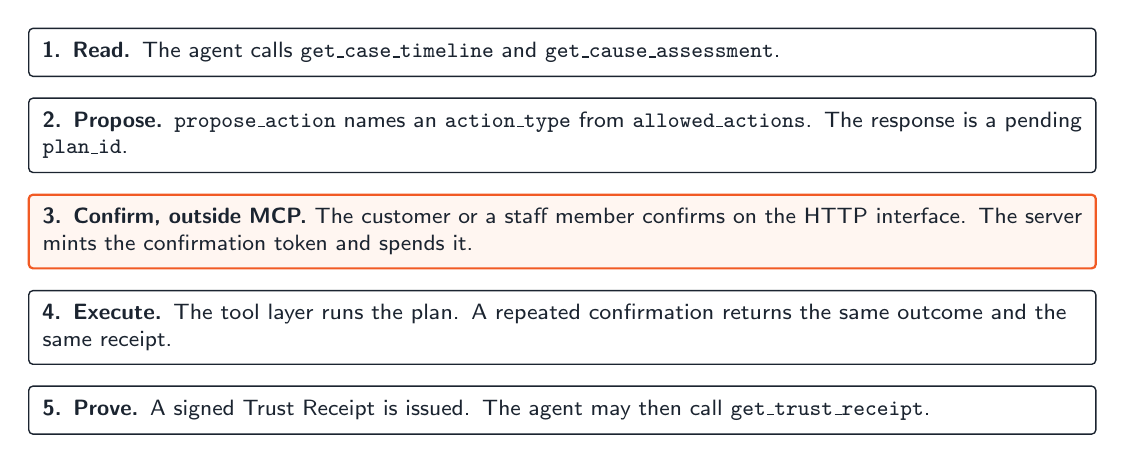
\begin{tikzpicture}[
  font=\sffamily\footnotesize,
  flow/.style={draw=hcNavy, line width=0.5pt, rounded corners=1.5pt,
               align=left, inner sep=5pt, fill=white, text width=132mm, text=hcNavy},
  hot/.style={flow, draw=hcOrange, line width=0.8pt, fill=hcWash}
]
  \node[flow] (s1) {\textbf{1. Read.} The agent calls \tool{get\_case\_timeline} and \tool{get\_cause\_assessment}.};
  \node[flow, below=2.6mm of s1] (s2) {\textbf{2. Propose.} \tool{propose\_action} names an \code{action\_type} from \code{allowed\_actions}. The response is a pending \code{plan\_id}.};
  \node[hot, below=2.6mm of s2] (s3) {\textbf{3. Confirm, outside MCP.} The customer or a staff member confirms on the HTTP interface. The server mints the confirmation token and spends it.};
  \node[flow, below=2.6mm of s3] (s4) {\textbf{4. Execute.} The tool layer runs the plan. A repeated confirmation returns the same outcome and the same receipt.};
  \node[flow, below=2.6mm of s4] (s5) {\textbf{5. Prove.} A signed Trust Receipt is issued. The agent may then call \tool{get\_trust\_receipt}.};
\end{tikzpicture}
\caption{The agent stops at a pending plan. Money moves only after confirmation, on a path the agent cannot call.}
\label{fig:sequence}
\end{figure}

\section{Denials}

Every call is audited, including a denial. The audit stores the tool name, safety level, principal, profile, case identifier, a hash of the arguments, the decision (\code{allowed}, \code{denied}, or \code{error}), and the error code. Argument values are hashed. They are not retained as customer text.

\begin{center}
\small
\begin{tabularx}{\textwidth}{@{}lX@{}}
\toprule
\textbf{Code} & \textbf{When it is returned} \\
\midrule
\code{UNKNOWN\_TOOL} & The name is not in the catalogue. \\
\code{NOT\_IN\_PROFILE} & The token's profile does not include the tool. \\
\code{INVALID\_ARGUMENTS} & A required argument is missing. \\
\code{AMOUNT\_NOT\_ACCEPTED} & The caller sent an amount. \\
\code{SESSION\_NOT\_BOUND} & A customer session has no case claim. \\
\code{NOT\_AUTHORISED\_FOR\_CASE} & The case is not the one in the token. \\
\code{LEVEL\_NOT\_EXPOSED} & The operation is L4. \\
\code{UNKNOWN\_RULE} & \tool{explain\_rule} was given an unknown rule. \\
\code{UNKNOWN\_ACTION} & \code{action\_type} is not in the action vocabulary. \\
\code{CASE\_NOT\_FOUND} & The case identifier does not exist. \\
\code{CASE\_NOT\_READY} & The case has no decision, or no receipt, for a tool that requires one. \\
\code{NO\_PROFILE\_SCOPE} & The token has no profile scope. \\
\code{AMBIGUOUS\_PROFILE} & The token has more than one profile scope. \\
\bottomrule
\end{tabularx}
\end{center}

A refusal the server expected is returned to the client as a tool error. An unauthenticated call ends at HTTP 401 and receives no tool result.

\section{Capabilities provided elsewhere}
\label{sec:outside}

The following are part of Hutch Clarity and are intentionally absent from \code{clarity-mcp}.

\begin{center}
\small
\begin{tabularx}{\textwidth}{@{}lX@{}}
\toprule
\textbf{Capability} & \textbf{Where it is provided} \\
\midrule
Confirm a plan & HTTP interface. Mints and spends the confirmation token. \\
Staff approval and step-up & HTTP interface, under the staff role. \\
Execute a refund or a service change & Tool layer, after a valid confirmation. \\
Sign and chain a Trust Receipt & Receipt service, on completion of a plan. \\
Auto-fix without a person & Deterministic path, only where the decision is \code{AUTO\_FIX}. Never from an agent. \\
Bulk remedy, policy publish, regulator export & Staff operations. Classed L4. Never over MCP. \\
Open a case and attach evidence & HTTP interface and the integration ports. \\
\bottomrule
\end{tabularx}
\end{center}

An integration that needs a registered agent to explain a charge, cite a rule, hand the case to a person, or propose an allowed remedy uses this specification. An integration that needs to confirm, approve, or execute uses the HTTP interface. Operator systems of record are reached through the integration ports, on the domain side of Figure~\ref{fig:doors}.

\section{Document control}

\begin{center}
\small
\begin{tabularx}{\textwidth}{@{}lllX@{}}
\toprule
\textbf{Version} & \textbf{Date} & \textbf{Status} & \textbf{Note} \\
\midrule
1.0 & 5 October 2026 & Issued & First issue of the MCP interface specification. Catalogue matches the ten tools provided by \code{clarity-mcp}. \\
\bottomrule
\end{tabularx}
\end{center}

\end{document}
